\documentclass[a4paper]{article}
\usepackage{graphicx}
\graphicspath{ {images/} }
\usepackage[english]{babel}
\usepackage[utf8]{inputenc}

\title{Merger Arbitrage Mid Term Report}

\author{Tianyuan Liu, Haoran Wang}

\date{\today}

\begin{document}
\maketitle

\section{Project Introduction}
\label{sec:idea}

One of the classic event-driven investment strategy in finance is called merger arbitrage. Every year, hundreds of public companies in the US are bought out (merged) by other companies. In order to successfully acquire the target company, the acquirer needs to pay a premium, which causes the target company’s share price to jump post-announcement. Since there is uncertainty regarding the success of the acquisition, the target’s post-announcement share price is usually below the acquirer’s offer price. This leads naturally to an investment strategy. If one can accurately predict the success/failure of the merger, one can buy the stocks that will succeed and short the stocks that will fail. Thus, our project goal is to create a model that predicts the success/failure of pending mergers.

\section{Data Description and Cleaning }
\label{sec:data}

Our data set primarily comes from SDC Platinum, a widely used M\&A database in corporate finance. We restrict our data to the years between 1990 and 2016, and only include those that involve a public entity as target. Non-public companies are excluded due to the lack of basic data like purchase price.

Originally, our data has 11678 data points (rows) and 29 features (columns). A shortened summary table of the features and brief description is available at the Appendix. The feature of interest is "Status". Status can take the following values: Completed, Dis Rumor, Intended, Part Comp, Pending, Rumor, Status Unknown, Withdrawn. To simplify our problem, we categorize all values other than "Completed" and "Pending" into "Failed", then we disregard all "Pending" values. Thus our problem becomes a binary classification problem. We further remove all data points that don't have "Price Per Share", the Acquiror's proposed acquisition price, or with a "Price Per Share" lower than \$1. This is standard practice in the finance literature and justified by the fact that without a known acquisition price, one has no way forming a trading strategy. Stocks that have a share price below \$ 1 usually exhibit funny behaviors and are often excluded from the analyze. We are now left with 8963 data points, which includes 7383 "Completed" and 1580 "Failed".

We then start creating features through feature transformation. Broadly speaking, the new features can be separated into three categories: Valuation, Deal Characteristic, Macro variables. The table below describes each variable. We also made histogram plots of various variables to get a sense of the variables distribution.


\begin{center}
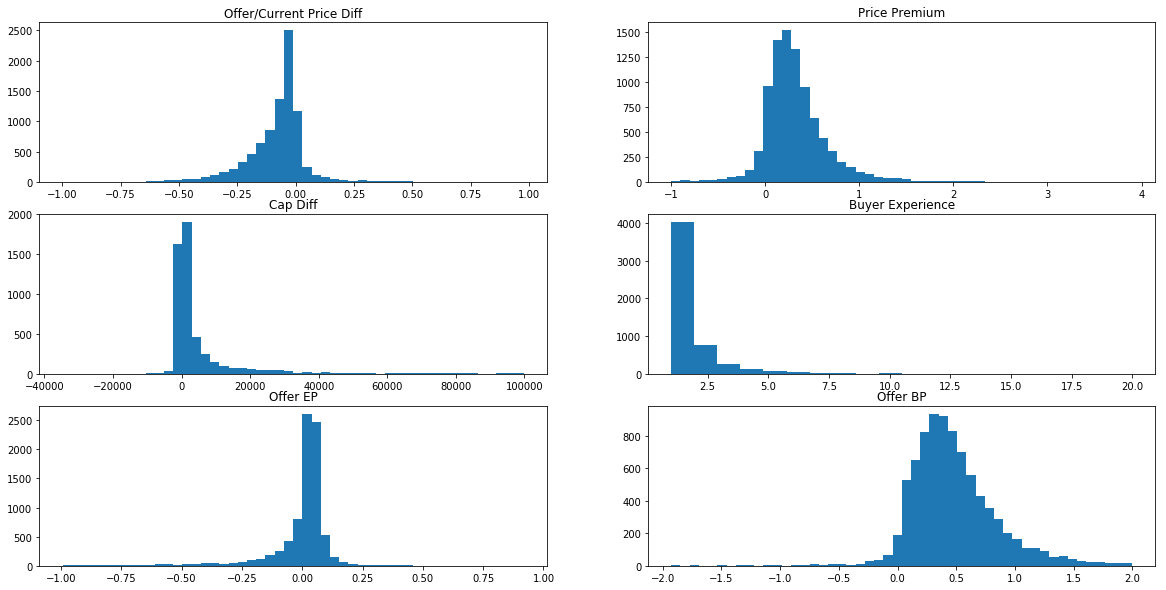
\includegraphics[scale=0.3]{hist.png} 
\end{center}

Additionally, like all financial data, the data set has many NaN. For example, nearly 1600 data points have a NaN for "Percent of Shares Acq.". Currently, we fill the NaN's with 0. It is likely worthwhile to investigate a better method in the future.


\section{Model Selection and Analysis }
\label{sec:model}

Before fitting the data with a model, we first need to specify what we are trying to outperform. Given the fact that we have more "Completed" than "Failed", we will aim to outperform a strategy that blindly guesses "Completed". Depending on how we split our training/validation/testing set, this benchmark ranges from 75% - 85%.

It is likely that many of the features are redundant. Thus we start our analysis using a logistic regression with L1 penalty. Unfortunately, the logistic model fails to outperform the benchmark; however, as expected, the lasso penalty quickly kills many features.

We next try a simple decision tree. We provide a illustrative graph below as an example of a possible split. It should be noted that three nodes only have 4 values, which is a dangerous sign of over fitting. 

\begin{center}
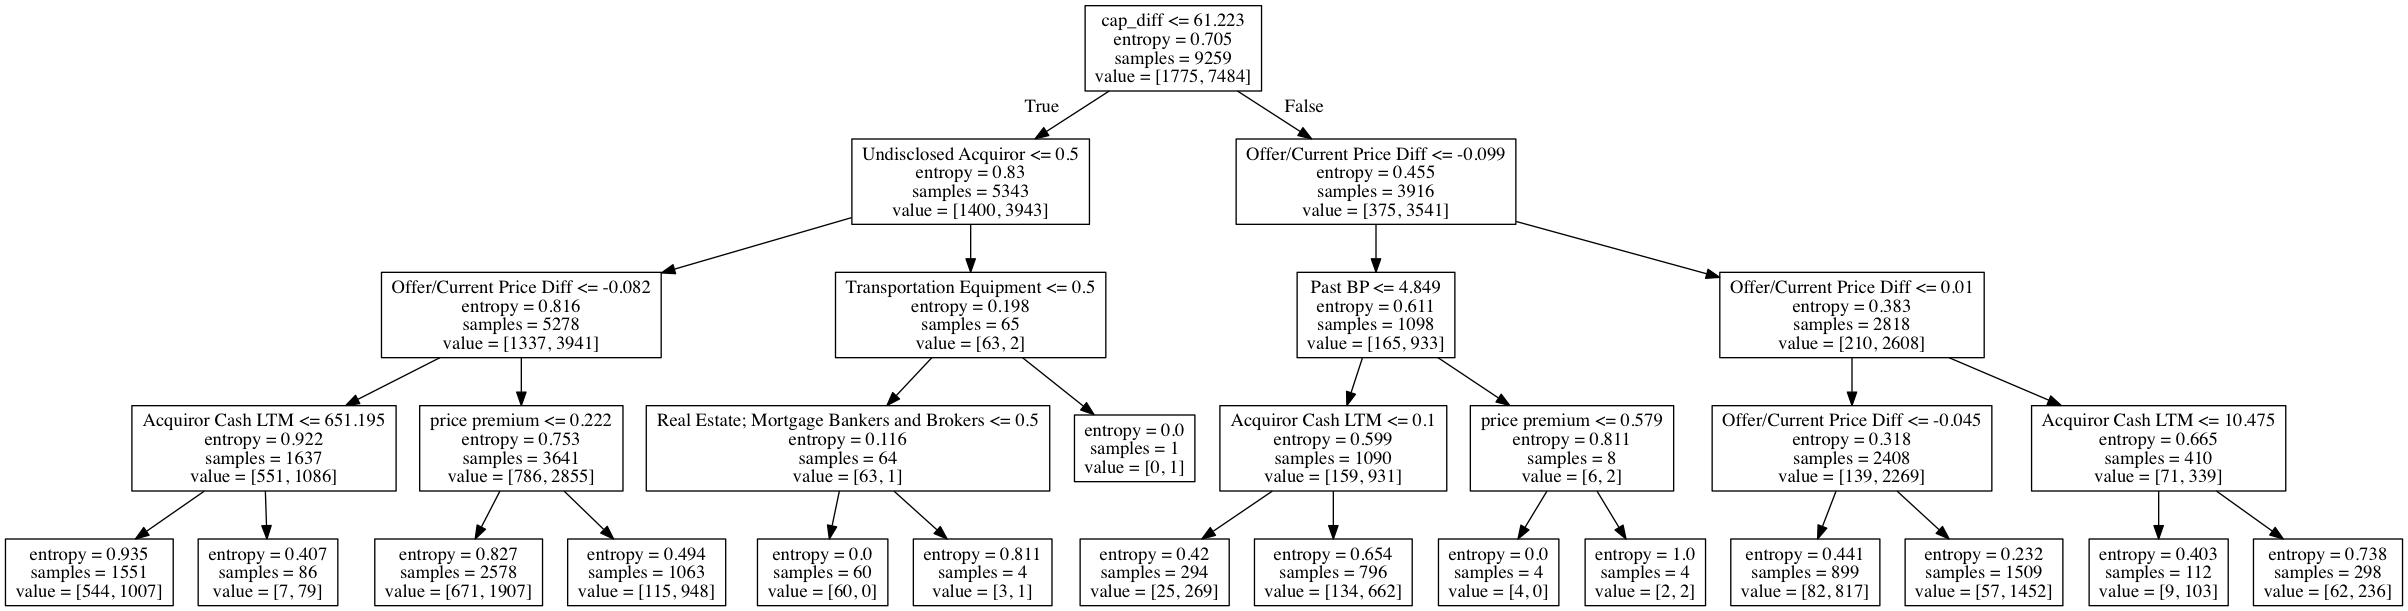
\includegraphics[scale=0.15]{tree.png} 

\end{center}

We then try a random forest classifier. Compared to a simple decision tree, a random forest classifier is much less prone to over-fitting. The random forest classifier performs slightly better. After choosing parameters using cross-validation, the model outperforms the benchmark by around 1 percent.  The random forest classifier also allows us to calculate the importance of each feature. We provide a bar chart below that shows the top 15 important features. Consistent with our intuition, "Offer/Current Price Diff" is the most important feature. 

\begin{center}
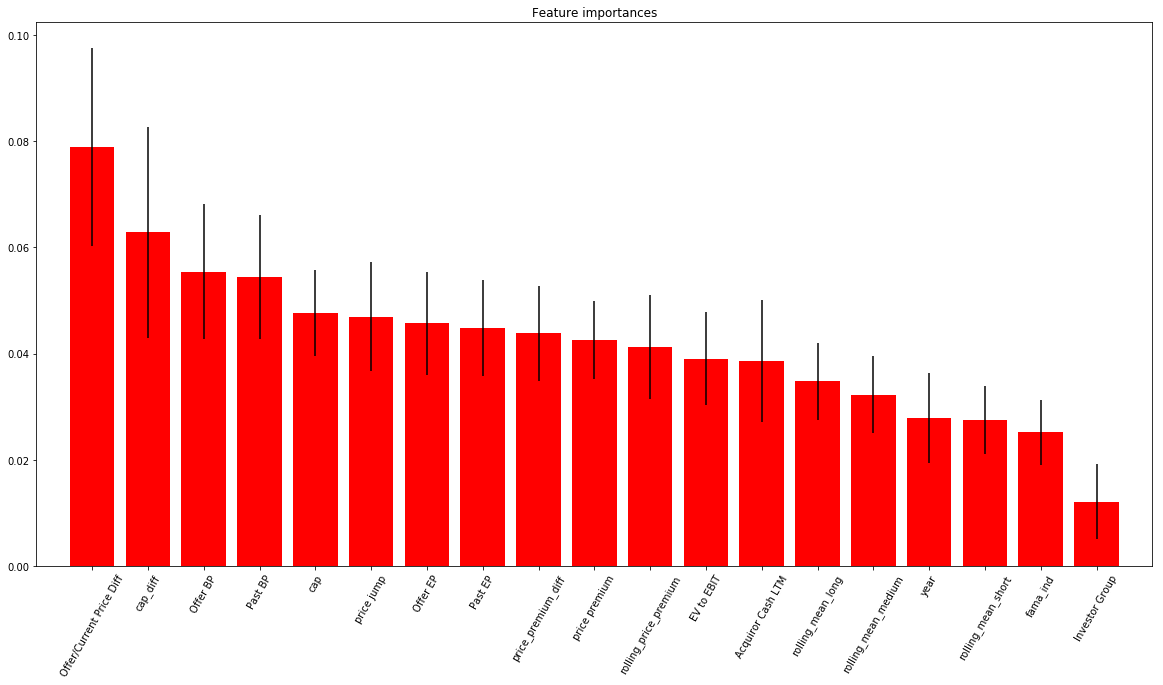
\includegraphics[scale=0.5]{Feature_Importance.png} 

\end{center}


\section{Future Steps }
\label{sec:future}

The current improvement over the benchmark is clearly unsatisfying. Going forward, we plan to introduce more features that potentially have predictive power. One feature that comes to mind is the implied volatility of the company's options before and after the merger announcement. This data can be found from OptionMetrics.

\newpage 
\section{Appendix }
\label{sec:tables}

\begin{table}[h]
\caption{Feature Description}
\begin{tabular}{ll}
Date Ann                 & Date of Merger Announcement                                  \\
Status                   & Final status of the deal                                     \\
\% of Shares Acq.        & \% of share the Acquiror aims to acquir                      \\
Price Per Share          & The price per share the Acquiror offers                      \\
Shares Out Actual        & Target's number of shares outstanding                        \\
Acquiror Cash LTM        & Acquiror's cash amount                                       \\
EV to EBIT               & Enterprise Value over Earning Before Interest and Tax        \\
Democrat/Republican      & Whether the deal happened during a Democrat presidency       \\
First Time               & Whether this is the first time the Acquiror has done a merger \\
Experienced              & more then 1 less then 20                            \\
nation diff              & Whether target and acquiror are from different nations       \\
industry diff            & Whether target and acquiror are from different industrys     \\
Offer/Current Price Diff & Offer price / price 1 day after announcement                 \\
Price Premium            & Offer price / price 1 day before announcement                \\
cap diff                & Capitalization difference between target and acquiror       
\end{tabular}
\end{table}

\end{document}
